\documentclass{article}
\usepackage[utf8]{inputenc}
\usepackage{graphicx}
\usepackage{minted}
%\usepackage{algorithm}
%\usepackage{algorithmic}
\graphicspath{ {images/} }
\makeatletter
\renewcommand\tableofcontents{%
    \@starttoc{toc}%
}
\makeatother

\title{Tabelle Hash}
\author{Vivoli Emanuele }
\date{8 Maggio 2017}

\begin{document}

\maketitle
\vspace*{0.33\textheight}
\tableofcontents

\newpage
\section{Introduzione}
Lo scopo dell'esercizio è studiare  le tabelle Hash che risolvono il problema delle collisioni ( quando due chiavi $key_1 \neq key_2$ sono associate alla stessa cella $h(key_1) = h(key_2)$ ) mediante le tecniche di Concatenamento ed Indirizzamento Aperto, e capire quale sia il comportamento delle tabelle Hash al crescere del fattore di carico $\alpha=\frac{n}{m}$ inserendo quindi in tabelle di dimensione $m$ una percetuale sempre maggiore di elementi $n$ , partendo dal $10\%$ di $m$ fino all'esaurimento delle celle libere inserendo il $100\%$ della dimensione della tabella.

La Funzione hash $h(k)$  è realizzata con la tecnica delle divisioni, un buon metodo poichè è veloce il calcolo della cella in cui inserire l'elemento.
La dimenisone della tabella hash con Indirizzamento Aperto e Concatenamento è il numero primo, rispettivamente maggiore e minore, più vicino ad $m$ valore dato ($num_p \leq m$ o $num_p \geq m$).

\newpage
\section{La Teoria}
\subsection{Tavola Hash}
La \textbf{Tavola Hash} è una struttura dati efficace per implementare dizionari (coppie $\{key : val\}$) ed è utilizzata al posto dell'Indirizzamento Diretto quando il numero di chiavi effettivamente memorizzate è piccolo rispetto al numero di chiavi appartenenti all'universo delle chiavi possibili.
\subsection{Funzione Hash}
Viene utilizzata una \textbf{Funzione hash} $h(x.key)$ per calcolare la cella della tavola nella quale inserire l'elemento $x$. Tale funzione puo essere implementata secondo due metodi: Divisioni e Moltiplicazioni; noi utilizzeremo il metodo delle Divisioni come richiesto dal testo, e dunque la Funzione hash sarà $h(k) = (k \% m)$.
Considereremo $m$ primo poiche se $m$ è una potenza intera del 2, utilizzando il metodo delle divisioni, si sfruttano solo un certo numero di bit della chiave e questo potrebbe non essere sufficente per ridurre il numero di collisioni e approssimare la funzione hash ad uniforme semplice.
\subsection{Collisioni}
Può darsi che a due chiavi distinte corrisponda la solita locazione all'interno della tabella Hash, e dunque si presenta un fenomeno chiamato \textbf{Collisione}. Queste posso essere risolte mediante due tecniche: Concatenamento e Indirizzamento Aperto.
A noi interessa di queste due implementazioni delle tabelle Hash la parte relativa all'inserimento. Vediemone le differenze:

\begin{description}
        \item[Concatenamento: ] ogni cella della tabella Hash è essa stessa una lista di elementi. L'inserimento avviene sempre in testa alla lista con un tempo di esecuzione $O(1)$. Si presenta una collisione ogni qualvolta la lista corrispondente alla cella nella quale si desidera inserire $x$ è non vuota.
            
        
        \item[Indirizzamento Aperto: ] la tabella Hash è composta da celle nelle quali puo essere inserito un solo elemento $x$. L'inserimento è tentato nella cella corrispondente a $h(x.key)$, se è non vuota allora viene ricalcolata una nuova cella mediante una funzione hash (nel nostro caso) a Ispezione Lineare: $h(k)=((x.key\%m)+i)\%m$.
        
        L'ispezione lineare consiste nel visitare le celle successive a $h(x.key)$ fino a che non si trova una cella libera nella quale inserire $x$, oppure abbiamo scorso tutta la tabella e dunque non vi è piu' posto per $x$, generando un overflow.
\end{description}
\newpage
\section{Aspettative}
Prima di studiare i risultati pratici che l'esecuzione del programma ci potrà mostrare, possiamo gia fare un'analisi riguardo al comportamento che ci aspettiamo.

La prima considerazione necessaria da fare riguarda il valore minimo delle liste di ispezione, che ci aspettiamo sia ad ogni percentuale $0$, dato che i primi elementi non produrranno alcuna lista di ispezione non genererando collisioni. 

Ci aspettiamo inoltre che all'aumentare del valore percentuale la lunghezza della lista di ispezione cresca, causata dal fenomeno chiamato "clustering primario". 

Alla percentuale massima ($100\%$) la lunghezza di ispezione è sempre non maggiore della dimensione della tabella, ma si avvicine molto ad essa ed anche se difficilmente raggiunge m, non si esclude comunque dai casi. 

Inoltre fino alle percentuali dell'$80\%$ ($\alpha=0.8$) la velocita di crescita della lista di ispezioni si manterrà bassa, crescendo però sproporzionalmente dopo tale percentuale intaccando in maniera significativa la sua performance.


\section{Descrizione esperimenti}
L'esperimento condotto ha lo scopo di capire quale sia il comportamento delle tabelle hash al crescere del fattore di carico $\alpha=\frac{n}{m}$, e dunque testiamo due tabelle che gestiscono in maniera differente le collisioni: Concatenamento e Indirizzamento Aperto.
La funzine hash utilizzata dalle due adotta il metodo delle divisioni, e come specificato sopra, è per questo che usiamo numeri primi come dimensione della tabella (se $m$ non è primo, c'è una funzione che ne calcola il numero primo immediatamente precedente o successivo).
\subsection{Dati utilizzati}
La dimensione $m$ iniziale è 1000, dunque nella tabella ad Indirizzamento aperto si avrà dimensione: 1009, mentre in quella con Concatenamento dimensione: 997.
Le percentuali da testare sono le seguenti:
[10, 20, 30, 40, 50, 60, 70, 75, 80, 85, 87, 89, 90, 91, 92, 93, 94, 95, 95, 97, 98, 99, 100]
Per ogni valore percentuale si effettuano 20 test, ed ogni test inserisce $m*(val\%)$ elementi nella tabella, contandone le collisioni ed aggiornando via via i valori di massimo, minimo e medio
Per l'Indirizzamento Aperto si calcolano anche le lunghezze di ispezione minime, massime e medie.

\newpage

\subsection{Codice di calcolo}

\inputminted{python}{python.py}

La funzione di start() della classe test è la funzione che esegue i test ed è caratterizzata da cicli interni, come possiamo vedere dal codice, che operano nel seguente modo:


Un ciclo che scorre la lista delle percentuali per ogni valore percentuale.


Un ciclo che esegue 20 test per ogni percentuale.


Ogni test deve creare una tabella ad Indirizzamento ed una con Concatenamento ed inserire nelle tabelle $m*(val\%)$ elementi x.


Gli elementi sono formati da chiave e valore random, dove la chiave è scelta con probabilità uniforme in un range da 0 a $100*m$.

Si conta se si sono presentate collisioni nella tabella ad Indirizzamento Aperto e nel caso si incrementa la variabile coll\_A.

Si controlla ed eventualmente si aggiornano i valori della lunghezza della sequenza di ispezioni minima, media e massima.


Aggiorno i valori di collisione minima, media e massima per la tabella ad Indirizzamento Aperto
aggiorno i valori di collisione minima, media e massima per la tabella con Concatenamento.
\newpage
\section{Documentazione}
Per l'esercizio sono utilizzati tre programmi che hanno i seguenti macro-ruoli:
\begin{itemize}
\item Un programma (hash.py) che implementa le tabelle hash
\item Un programma (test.py) che conta quante collisioni si hanno eseguendo un numero variabile di inserimenti in una tabella hash
\item Un programma (exp.py) che esegue gli esperimenti
\end{itemize}

Il programma \textbf{hash.py} implementa la classe Node (gli oggetti che si vogliono inserire) composta da chiave e valore; la classe Hash\_IA che corrisponde alla tabella ad Indirizzamento Aperto composta da un attributo unico 'coll', che conta per ogni inserimento la lunghezza della lista di ispezione per quell'inserimento; la classe Hash\_C che corrisponde alla tabella per Concatenamento composta anche essa da un unico attributo 'coll' che conta quante collisioni ci sono state per tutti gli inserimenti fatti nella tabella fino ad ora.
Le classi Hash hanno anche tutte le operazioni base della struttura dati (inserimento, cancellazione, ricerca, ecc..). 

Il programma \textbf{test.py} implementa la classe 'Coll' (oggetto Collisione per ogni percentuale) formata dagli attributi min\_, med\_, max\_; la classe 'Len\_Ispection' (oggetto Lunghezza di ispezione per ogni percentuale) che riguarda solo le tabelle ad Indirizzamento aperto formata dagli attributi min\_, med\_, max\_. C'è inoltre la classe 'test' che esegue i cicli sopra desctritti e trova per ogni percentuale i valori desiderati.
Il programma test.py prende in input una stringa, corrispondente al nome del file pickle nel quale è memoriazzata una lista formata da due elementi: la dimensione delle tabelle e una lista di valori percentuali. Il programma trasforma in un oggetto il file pickle, esegue i calcoli dovuti e crea al termine un nuovo file pickle con sopra memorizzata una lista di eementi dove il primo corrisponde alla lista delle percentuali, ed i successivi sono liste con il valore minimo, medio e massimo dei collisioni, e quando richiesto anche lunghezza della lista di ispezione, per ogni percentuale. il programma restituisce il titolo del file pickle contenete il risultato.

Il programma \textbf{exp.py} crea un file pickle, crea un oggetto test e gli passa il nome del file, prende il file pickle che test ha creato e lo salva in un oggetto e 'plotta' l'andamento delle collizioni e lunghezza della lista di ispezioni per ogni valore percentuale testato. 

\newpage
\section{Risultati Sprimentali}
\subsection{Indirizzamento Aperto}

\begin{center}
    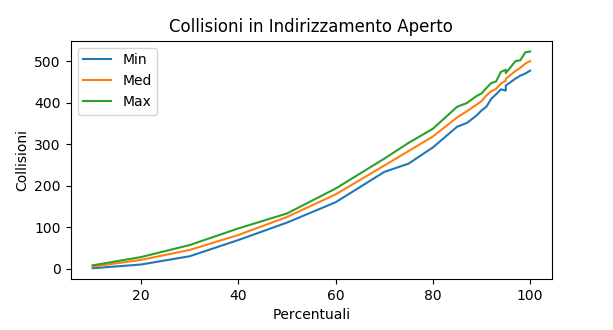
\includegraphics[scale=0.8]{IA_Coll.png}
    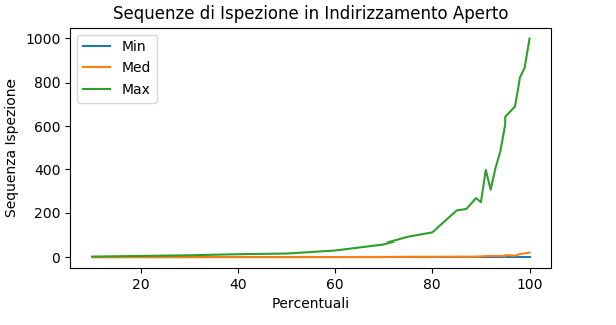
\includegraphics[scale=0.8]{IA_LenI.png}
\end{center}




Iniziamo parlando delle tabelle ad \textbf{indirizzamento aperto}, dove svolgiamo due calcoli differenti: il valore minimo, medio e massimo delle collisioni ed il valore minimo, medio e massimo della lunghezza della sequenza di ispezione; valori misurati nell'inserimento di percentuali sempre maggiori di elementi (partiamo inserendo $10\%$, $20\%$, e sempre crescendo fino al $100\%$ di $m$ dimensione della tabella).

Una collisione corrisponde al primo tentativo di inserire l'elemento $x$ all'interno della tabella hash. 

Se la cella non è libera si tenta l'inserimento nelle locazioni consecutive calcolate dalla funzione hash e definiamo la lunghezza della lista di ispezione per un determinato inserimento di un elemento $x$ il numero totale di ricalcoli a partire dal primo tentativo.

Poiche viene richiesto di calcolare tali misure su 20 test per ogni valore percentuale data dal testo, si procede via via ad aggiornare le misure di minimo, medio e massimo per le collisioni e per le liste di ispezione, considerando, inoltre, come media totale la media su ognuna delle prove, mediata successivamente sulle 20 prove per valore percentuale.

L'esperimento ha reso i risultati che avevamo ipotizzato per la lunghezza della lista di ispezione riguardo all'hashing con Indirizzamento Aperto, e dunque si è presentato, ed è possibile visualizzarlo dal grafico, il fenomeno di clustering primario cioè (nel nostro caso cui interessa solamente l'inserimento) la formazione di lunghe code che rallentano la ricerca della cella in cui inserire il dato.
Possiamo anche fare una considerazione a posteriori notando come questo fenomeno sia visibile solo andando a vedere i valori massimi raggiunti in un test d'inserimento e che in media è un problema che riguarda le percentuali vicine al $100\%$ (infatti nel grafico il valor medio della lunghezza di ispezione alla percentuale del $100\%$ arriva ad un valore di 20, non esagerato rispetto ai 1000 elementi inseriti, e molto minore rispetto al valor massimo misurato).

\subsection{Concatenamento}

\begin{center}
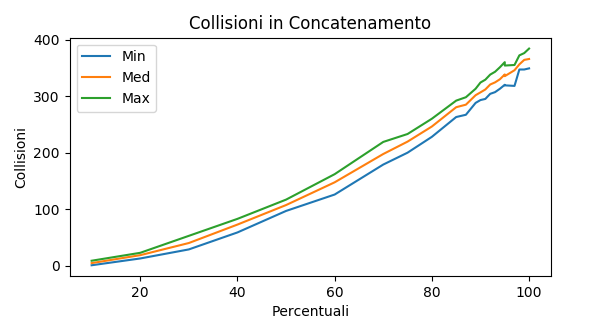
\includegraphics[scale=0.8]{C_Coll.png}
\end{center}

Riguardo alle tabelle hash con \textbf{concatenamento}, l'obiettivo è quello di calcolare solamente il valore minimo, medio e massimo delle collisioni, cioè il numero di collisioni che si presentano inserendo un elemento in testa alla coda relativa alla cella calcolata dalla funzione hash, quando la lista è non vuota.
Possiamo immediatamente notare dai grafici come all'aumentare del valore percentuale aumenti anche il numero di collisione minimo e massimo, quindi anche medio che li segue e ne è limitato.

%
%	INSERIRE DELLE TABELLE:
%		INDIRIZZAMENTO APERTO
%		CONCATENAMENTO
%

\end {document}